% LaTeX version of the SMD-UTM 2026 paper template (Conferința Tehnico-Științifică a Studenților,
% Masteranzilor și Doctoranzilor, Universitatea Tehnică a Moldovei). Compile with XeLaTeX (Overleaf:
% Menu -> Compiler -> XeLaTeX). Times New Roman is used if installed, otherwise its free clone TeX Gyre Termes.
\documentclass[12pt,a4paper]{article}

% ---- page: A4 portrait; top, bottom, right 2.0 cm, left 2.5 cm (template rule)
\usepackage[a4paper,top=2cm,bottom=2cm,right=2cm,left=2.5cm,headheight=46pt,headsep=14pt,
            footskip=38pt,includeheadfoot=false]{geometry}

% ---- fonts: Times New Roman 12 pt
\usepackage{amsmath,amssymb}
\usepackage{fontspec}
\IfFontExistsTF{Times New Roman}{\setmainfont{Times New Roman}}{\setmainfont{TeX Gyre Termes}}
\usepackage[provide=*,romanian]{babel}

% ---- paragraphs: single spacing, every paragraph indented 1.25 cm
\setlength{\parindent}{1.25cm}
\setlength{\parskip}{0pt}
\usepackage{indentfirst}
\usepackage{microtype}

% ---- headings: bold 12 pt, indented 1.25 cm, not numbered, blank line before
\usepackage{titlesec}
\setcounter{secnumdepth}{0}
\titleformat{\section}{\normalfont\normalsize\bfseries}{}{0pt}{\hspace*{1.25cm}}
\titlespacing*{\section}{0pt}{12pt}{0pt}
\titleformat{\subsection}{\normalfont\normalsize\bfseries\itshape}{}{0pt}{\hspace*{1.25cm}}
\titlespacing*{\subsection}{0pt}{6pt}{0pt}

% ---- figures: centred; caption below, "Figura n." bold, 11 pt, centred
\usepackage{graphicx,float}
\usepackage[font={small,bf},labelfont=bf,labelsep=period,justification=centering,skip=4pt]{caption}
\captionsetup[figure]{name=Figura}
\setlength{\abovecaptionskip}{4pt}

% ---- tables: 10 pt, full width, all borders
\usepackage{array,tabularx}
\renewcommand{\arraystretch}{1.15}

% ---- lists, links
\usepackage{enumitem}
\usepackage{setspace}
\usepackage[hidelinks]{hyperref}
\usepackage{xurl}
\providecommand{\tightlist}{\setlength{\itemsep}{0pt}\setlength{\parskip}{0pt}}

% ---- header (UTM logo + conference) and footer (place, date, volume, page number)
\usepackage{fancyhdr}
\pagestyle{fancy}
\fancyhf{}
\renewcommand{\headrulewidth}{0.6pt}
\renewcommand{\footrulewidth}{0.6pt}
\fancyhead[L]{\raisebox{-2pt}{
\includegraphics[height=1.55cm]{logo_utm.png}}}
\fancyhead[C]{\parbox[b]{12cm}{\centering\fontsize{11}{13}\selectfont\itshape
  Conferința Tehnico-Științifică a Studenților, Masteranzilor și Doctoranzilor\\
  Universitatea Tehnică a Moldovei\vspace{2pt}}}
\fancyfoot[C]{{\fontsize{11}{13}\selectfont\itshape Chișinău, 13-16 Mai, 2026, Vol. N}\\[2pt]
  {\fontsize{11}{13}\selectfont - \thepage\ -}}

\begin{document}
\raggedbottom
\begin{center}
{\fontsize{14}{16}\selectfont\bfseries DESCOMPUNEREA BAYESIANĂ A INCERTITUDINII PENTRU AVERTIZAREA TIMPURIE A DEVIERII CONCEPTUALE, VALIDATĂ PRIN XAI\par}
\vspace{12pt}
{\bfseries Prenumele NUMELE\textsuperscript{1*}\par}
\vspace{10pt}
{\fontsize{10}{12}\selectfont\itshape \textsuperscript{1}Departamentul [denumirea], grupa [grupa], Facultatea [denumirea], Universitatea Tehnică a Moldovei, Chișinău, Republica Moldova\par}
\vspace{10pt}
{\fontsize{10}{12}\selectfont *Autorul corespondent: Prenumele Numele, [e-mail]\par}
\vspace{10pt}
{\fontsize{10}{12}\selectfont\bfseries Îndrumătorul/coordonatorul științific \normalsize Prenumele NUMELE\fontsize{10}{12}\selectfont, \mdseries [titlul științific, afilierea]\par}
\end{center}
\vspace{6pt}

{\itshape\let\emph\textit

\noindent \textbf{\emph{Rezumat.}} Detectoarele clasice de deviere
conceptuală urmăresc rata de eroare a modelului, deci au nevoie de
etichete și reacționează abia după ce acuratețea a scăzut. Lucrarea
testează dacă incertitudinea modelului, calculată numai din intrări,
poate da o alarmă mai devreme și ce componentă a ei este utilă. Entropia
predictivă a unei rețele MC-Dropout, a unui ansamblu de rețele și a două
ansambluri frecventiste (SVM și pădure aleatoare) este separată în
incertitudine aleatorică și epistemică, iar raportul lor logaritmic este
propus ca semnal de monitorizare. Pe 225 de fluxuri construite din date
reale, cu moment de deviere cunoscut, și pe fluxul natural Elec2, cinci
ipoteze stabilite în prealabil au fost testate statistic. Raportul
separă cel mai bine datele deviate pentru rețelele neuronale (aria de
sub curba ROC 0.80 față de 0.67), dar nu și pentru modelele
frecventiste. Alarma fără etichete vine mai devreme decât detectoarele
bazate pe eroare, însă precede scăderea vizibilă a acurateței doar în 51
\% din cazuri. Devierea relației dintre intrări și etichete rămâne
invizibilă fără etichete, iar SHAP, spre deosebire de LIME, indică
trăsăturile care au deviat. Codul și datele permit reproducerea
integrală.

\par}

\vspace{12pt}{\itshape\let\emph\textit

\noindent \textbf{\emph{Cuvinte cheie:}} \emph{informație mutuală, monte
carlo dropout, monitorizare fără etichete, valori shapley, inferență
statistică.}

\par}

\hypertarget{introducere}{%
\section{Introducere}\label{introducere}}

Un model de învățare automată este antrenat pe date istorice și apoi
folosit pe date noi, a căror distribuție
\(P_t(x,y)=P_t(x)\,P_t(y\mid x)\) se schimbă în timp. Fenomenul se
numește deviere conceptuală (\emph{concept drift}) {[}1,2{]}.
Detectoarele uzuale, DDM (\emph{Drift Detection Method}) {[}3{]}, ADWIN
(\emph{ADaptive WINdowing}) {[}4{]} și Page-Hinkley (PH) {[}5{]},
urmăresc rata de eroare. Ele au nevoie de eticheta reală a fiecărei
predicții, care în creditare sau în detectarea fraudei sosește după
luni, și reacționează după ce acuratețea a scăzut.

O alternativă este incertitudinea modelului însuși. Baier et al.~{[}6{]}
monitorizează incertitudinea \emph{totală} a unei rețele Monte Carlo
Dropout (MC-Dropout). Teoria bayesiană permite însă separarea
incertitudinii în componenta aleatorică (AU, zgomotul din date) și cea
epistemică (EU, ignoranța modelului) {[}7--9{]}. Contribuțiile lucrării
sunt: (i) raportul \(\log(EU/AU)\) ca semnal de monitorizare, comparat
direct cu componentele sale; (ii) demonstrarea limitei oricărei detecții
fără etichete; (iii) validarea alarmelor prin metode de inteligență
artificială explicabilă (XAI): explicarea funcției \(EU(x)\) cu SHAP
(\emph{SHapley Additive exPlanations}) și LIME (\emph{Local
Interpretable Model-agnostic Explanations}); (iv) comparația dintre
incertitudinea bayesiană și cea frecventistă; (v) fluxuri semi-sintetice
cu moment și trăsături de deviere cunoscute.

Ipotezele, fixate înainte de experimente, sunt: \textbf{H1} -- sub
devieri ale lui \(P(x)\), alarma pe \(\log(EU/AU)\) precede scăderea
vizibilă a acurateței; \textbf{H2} -- raportul separă datele deviate mai
bine decât EU, AU, entropia totală (TU) și \(1-\max p\); \textbf{H3} --
sub deviere pură a lui \(P(y\mid x)\) niciun semnal de incertitudine nu
conține informație; \textbf{H4} -- atribuirile SHAP/LIME ale lui EU
indică trăsăturile deviate; \textbf{H5} -- incertitudinea bayesiană și
cea frecventistă se comportă diferit.

\hypertarget{metodologie}{%
\section{Metodologie}\label{metodologie}}

\hypertarget{modele-ux219i-descompunerea-incertitudinii}{%
\subsection{Modele și descompunerea
incertitudinii}\label{modele-ux219i-descompunerea-incertitudinii}}

Antrenarea prin entropie încrucișată este o estimare de verosimilitate
maximă, iar penalizarea L2 corespunde unei distribuții a priori
gaussiene (estimare \emph{maximum a posteriori}, MAP). Rețelele au două
straturi ascunse de 64 de neuroni cu activare ReLU (\emph{rectified
linear unit}). Distribuția a posteriori a ponderilor este aproximată
prin MC-Dropout cu \(T=30\) măști fixe {[}10{]} și printr-un ansamblu de
\(M=5\) rețele {[}11{]}. Ca termen frecventist se folosesc 10 mașini cu
vectori-suport (SVM) cu nucleu gaussian (RBF), antrenate pe eșantioane
bootstrap. Ca analiză suplimentară, adăugată după studiul principal, se
folosește o pădure aleatoare de 50 de arbori {[}12{]}, descompusă ca în
{[}13{]}. Pentru \(S\) distribuții predictive eșantionate \(p_s\),
descompunerea {[}8{]} este dată de Ec. (1):

\begin{equation}
\underbrace{H\Big[\frac{1}{S}\sum_{s} p_s\Big]}_{TU} = \underbrace{\frac{1}{S}\sum_{s} H[p_s]}_{AU} + \underbrace{I(y;\theta \mid x)}_{EU}
\end{equation}

unde \(H\) este entropia, iar \(I\) este informația mutuală dintre
etichetă și parametri. EU este mare când modelele eșantionate nu sunt de
acord. Semnalul propus este dat de Ec. (2), cu \(\varepsilon=10^{-4}\):

\begin{equation}
LR(x)=\log\big(EU(x)+\varepsilon\big)-\log\big(AU(x)+\varepsilon\big)
\end{equation}

Dacă \(P_t(x)\) rămâne constant, orice funcție \(g(x)\), inclusiv EU, AU
și LR, are aceeași distribuție înainte și după deviere, deci un detector
bazat pe ea nu poate depăși nivelul de semnificație. Această limită este
testată prin H3.

\hypertarget{date-ux219i-fluxuri-cu-deviere-cunoscutux103}{%
\subsection{Date și fluxuri cu deviere
cunoscută}\label{date-ux219i-fluxuri-cu-deviere-cunoscutux103}}

Seturile de date sunt prezentate în Tab. 1. Toate sunt publice, au
licențe care permit cercetarea și sunt verificate prin amprentă SHA-256
la fiecare rulare.

\begin{flushright}\textit{\fontsize{11}{13}\selectfont Tabelul 1}\end{flushright}\vspace{-6pt}
\begin{center}{\fontsize{11}{13}\selectfont\bfseries Seturile de date utilizate}\end{center}\vspace{-6pt}
{\fontsize{10}{12}\selectfont
\begin{tabularx}{\textwidth}{|>{\raggedright\arraybackslash}X|>{\raggedright\arraybackslash}p{2.9cm}|>{\centering\arraybackslash}p{2.6cm}|>{\raggedright\arraybackslash}p{3.2cm}|>{\raggedright\arraybackslash}p{2.1cm}|}
\hline
\textbf{Set de date} & \textbf{Domeniu} & \textbf{Înregistrări × trăsături} & \textbf{Țintă (rata clasei pozitive)} & \textbf{Licență}\\\hline
Credit (Taiwan, 2005) [14] & risc de credit & 30 000 × 23 & neplată (22.1 \%) & CC BY 4.0\\\hline
Telco Customer Churn [15] & clienți telecom & 7 043 × 19 & plecarea clientului (26.5 \%) & Apache-2.0\\\hline
Elec2 [16] & piața energiei, flux natural & 45 312 × 6 & creșterea prețului (42.5 \%) & liberă pentru cercetare\\\hline
Cifre 8×8 (UCI) & imagini & 1 797 × 64 & 10 clase & CC BY 4.0\\\hline
SEA [17] & sintetic & generat & binar & generat cu River [18]\\\hline
\end{tabularx}}
\vspace{6pt}

Pentru a putea măsura avansul unei alarme, fiecare set real este
transformat într-un flux: 3 000 de înregistrări pentru antrenare, 1 000
pentru calibrare și un flux de 6 000, în care devierea începe la
înregistrarea 2 500 și crește liniar pe 1 500 de înregistrări. Au fost
generate patru mecanisme: \emph{covariată} (un segment nou de clienți,
\(P(x)\)), \emph{senzor} (două trăsături deplasate cu \(2\sigma\)),
\emph{reală} (etichete inversate cu probabilitatea 0.7 într-o regiune,
\(P(y\mid x)\)) și \emph{fără deviere} (pentru alarme false).
Trăsăturile deviate sunt înregistrate. Datele nu conțin identificatori
personali, iar singurele valori lipsă (0.16 \% din coloana
\emph{TotalCharges} a setului Telco) au fost imputate cu mediana.
Populația o constituie toate înregistrările unui set, iar eșantioanele
de antrenare, calibrare și flux sunt extrase cu semințe fixe (0--4).

\hypertarget{detectori-evaluare-ux219i-inferenux21bux103}{%
\subsection{Detectori, evaluare și
inferență}\label{detectori-evaluare-ux219i-inferenux21bux103}}

Semnalele fără etichete sunt monitorizate cu PH, ADWIN, o detecție
bayesiană online a punctelor de schimbare (BOCPD) {[}19{]} și un amestec
gaussian estimat prin algoritmul \emph{Expectation-Maximization} (EM)
{[}20{]}, ultimele două implementate de autor, alături de testul
Kolmogorov-Smirnov pe intrări {[}21{]}. Pragurile sunt calibrate astfel
încât probabilitatea unei alarme false pe un flux staționar să fie cel
mult 0.10. Scăderea vizibilă a acurateței este primul moment în care
acuratețea pe ultimele 300 de înregistrări scade cu peste trei erori
standard sub nivelul inițial. Separabilitatea unui semnal este măsurată
prin aria de sub curba ROC (AUROC; 0.5 înseamnă nicio informație).
Atribuirile sunt calculate cu KernelSHAP {[}22{]}, GradientSHAP și LIME
{[}23{]}.

Înregistrările dintr-un flux nu sunt independente, de aceea unitatea de
analiză este rularea. Au fost efectuate 225 de rulări (12 scenarii × 3
modele × 5 semințe, plus 45 de ablații), testate cu Wilcoxon și corecție
Holm {[}24{]}, echivalența cu hazardul prin testul TOST (\emph{two
one-sided tests}) {[}25{]}, fluxul Elec2 prin bootstrap pe blocuri
{[}26{]}, iar rezultatele pe seturi de date au fost agregate prin
meta-analiză cu efecte aleatoare {[}27{]}. Toți parametrii se află
într-un singur fișier de configurare, iar rezultatele au fost reproduse
identic pe o copie nouă a depozitului.

\hypertarget{rezultate-ux219i-discuux21bii}{%
\section{Rezultate și discuții}\label{rezultate-ux219i-discuux21bii}}

Fig. 1 prezintă o rulare tipică. Odată cu devierea, AU \emph{scade}, iar
EU crește. Alarma pe LR apare la 6 înregistrări înaintea scăderii
vizibile și cu 200 înaintea primului detector bazat pe eroare.

\begin{figure}[H]\centering
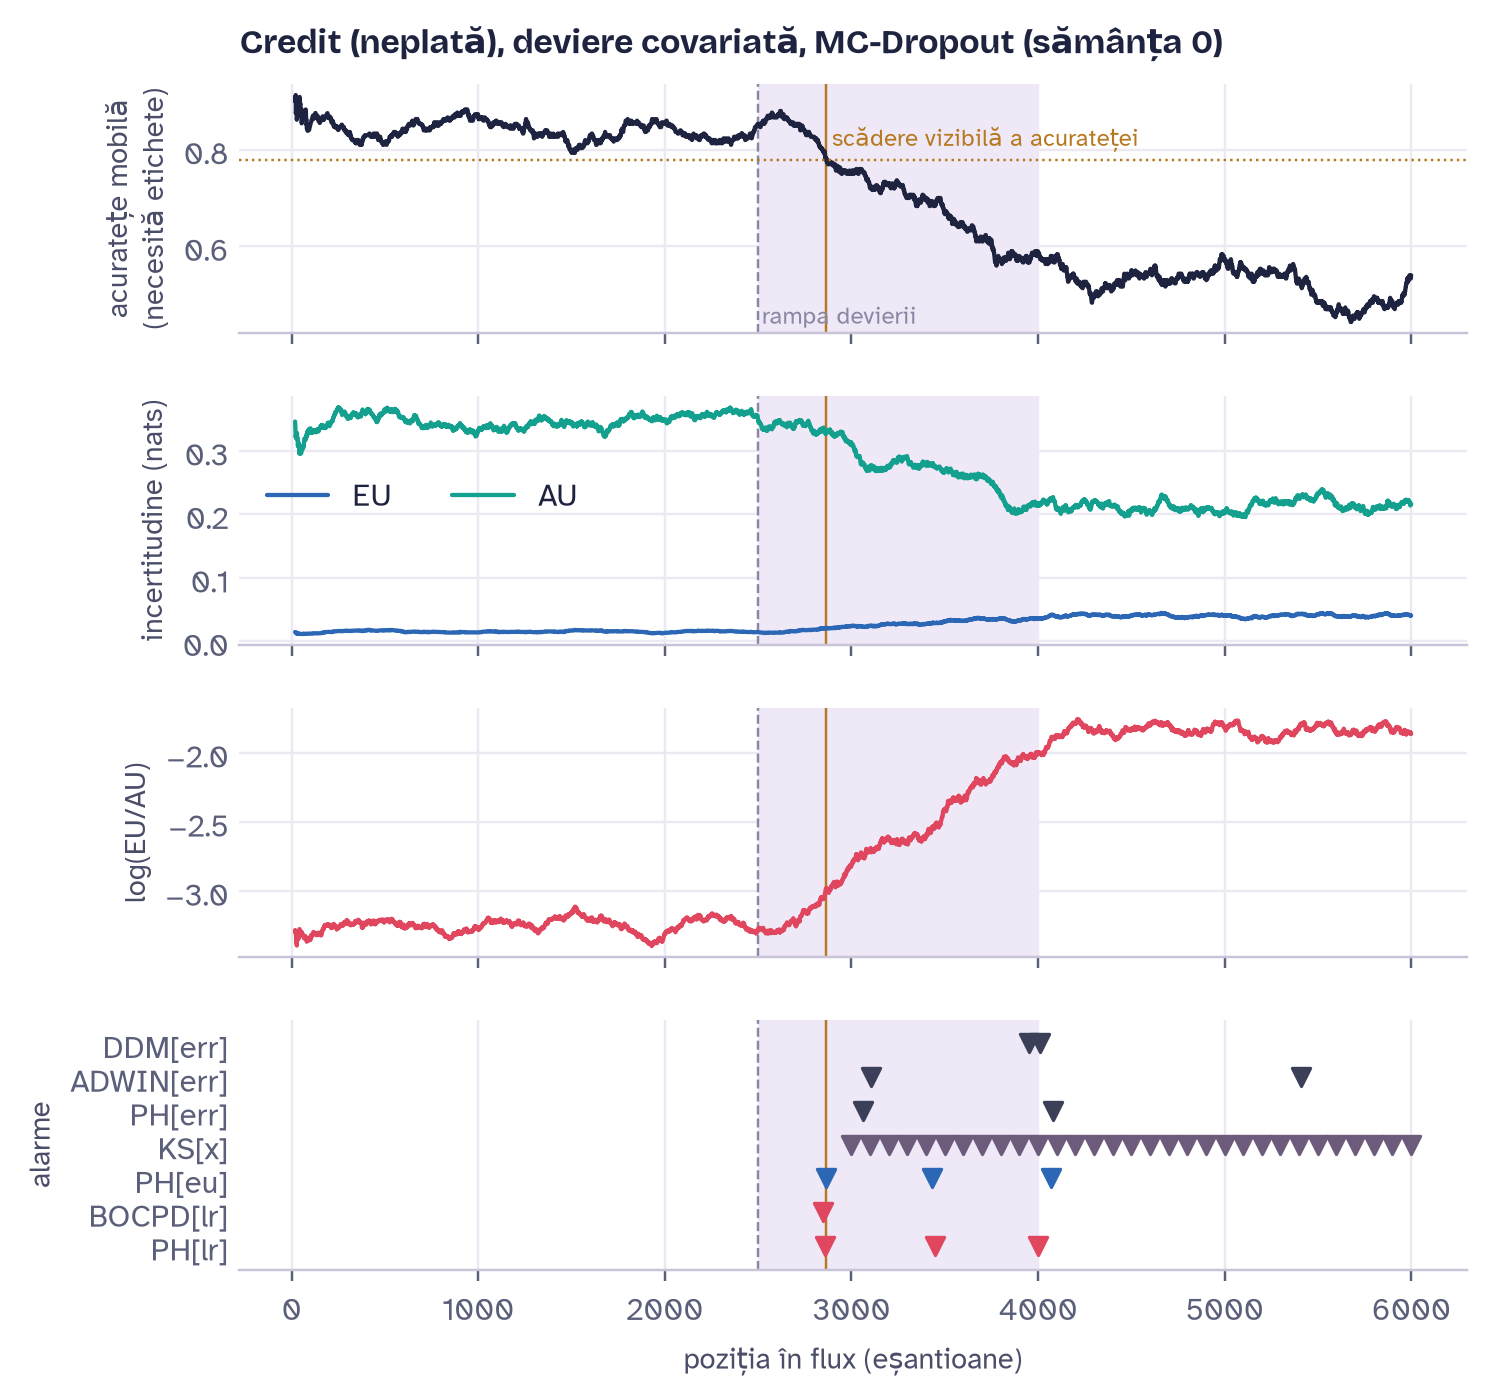
\includegraphics[width=16cm]{figures/fig1_example_trace.png}
\caption{Credit, deviere covariată, MC-Dropout: acuratețea, AU și EU, semnalul LR și alarmele detectorilor}
\end{figure}

\textbf{H2 este confirmată.} Pe devierile lui \(P(x)\), LR are AUROC
median 0.80, față de 0.67 pentru EU, 0.53 pentru TU, 0.50 pentru AU și
0.53 pentru \(1-\max p\) (toate comparațiile: \(p_{Holm}<0.001\); Fig.
2). Sub deviere reală, toate semnalele au AUROC 0.50 și sunt echivalente
statistic cu hazardul (TOST, \(p<0.001\)), în timp ce detectoarele
bazate pe eroare detectează 100 \% din devieri. \textbf{H3 este
confirmată}, așa cum prezice limita teoretică.

\begin{figure}[H]\centering
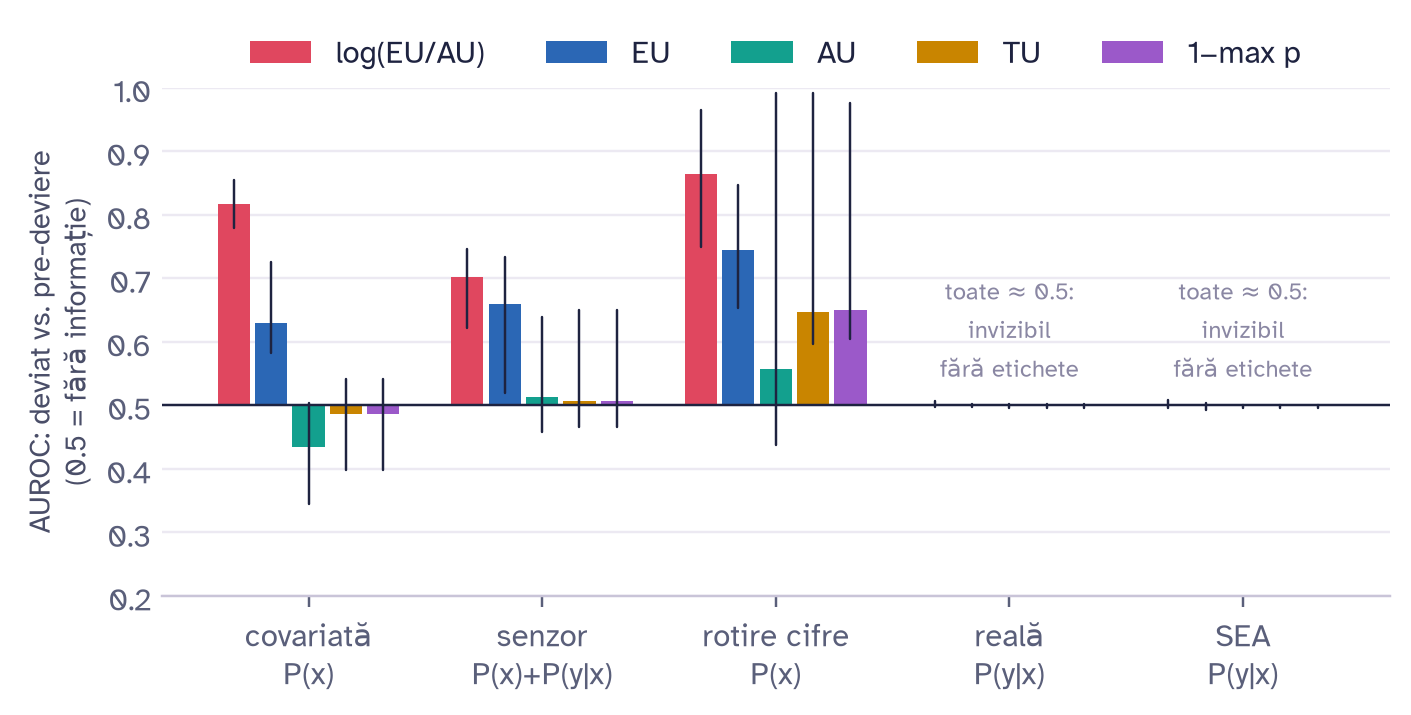
\includegraphics[width=15cm]{figures/fig2_signal_auroc.png}
\caption{Separabilitatea fiecărui semnal (AUROC median, interval de încredere 95 \%) pe tipuri de deviere}
\end{figure}

\textbf{H5: avantajul raportului depinde de model} (Tab. 2, Fig. 3).
Pentru rețele, LR este cel mai bun semnal, deoarece rețelele ReLU devin
supra-încrezătoare departe de datele de antrenare {[}28{]}: AU scade, EU
crește, iar logaritmul raportului le însumează. SVM-ul și pădurea
aleatoare revin spre predicții moderate, AU crește odată cu EU, iar
raportul pierde.

\begin{flushright}\textit{\fontsize{11}{13}\selectfont Tabelul 2}\end{flushright}\vspace{-6pt}
\begin{center}{\fontsize{11}{13}\selectfont\bfseries AUROC median pe devierile $P(x)$ și testul pereche LR vs.\ EU (Holm)}\end{center}\vspace{-6pt}
{\fontsize{10}{12}\selectfont
\begin{tabularx}{\textwidth}{|>{\raggedright\arraybackslash}X|c|c|c|c|>{\centering\arraybackslash}p{2.4cm}|c|}
\hline
\textbf{Model} & \textbf{LR} & \textbf{EU} & \textbf{AU} & \textbf{TU} & \textbf{Cazuri cu LR > EU (\%)} & \textbf{p (Holm)}\\\hline
MC-Dropout (bayesian aprox.) & 0.811 & 0.629 & 0.382 & 0.454 & 80 & 0.0003\\\hline
Ansamblu profund (bayesian aprox.) & 0.826 & 0.672 & 0.426 & 0.486 & 92 & < 0.001\\\hline
SVM bootstrap (frecventist) & 0.611 & 0.779 & 0.699 & 0.713 & 12 & < 0.001\\\hline
Pădure aleatoare (frecventist, analiză suplimentară) & 0.613 & 0.775 & 0.681 & 0.713 & 4 & < 0.001\\\hline
\end{tabularx}}
\vspace{6pt}

\begin{figure}[H]\centering
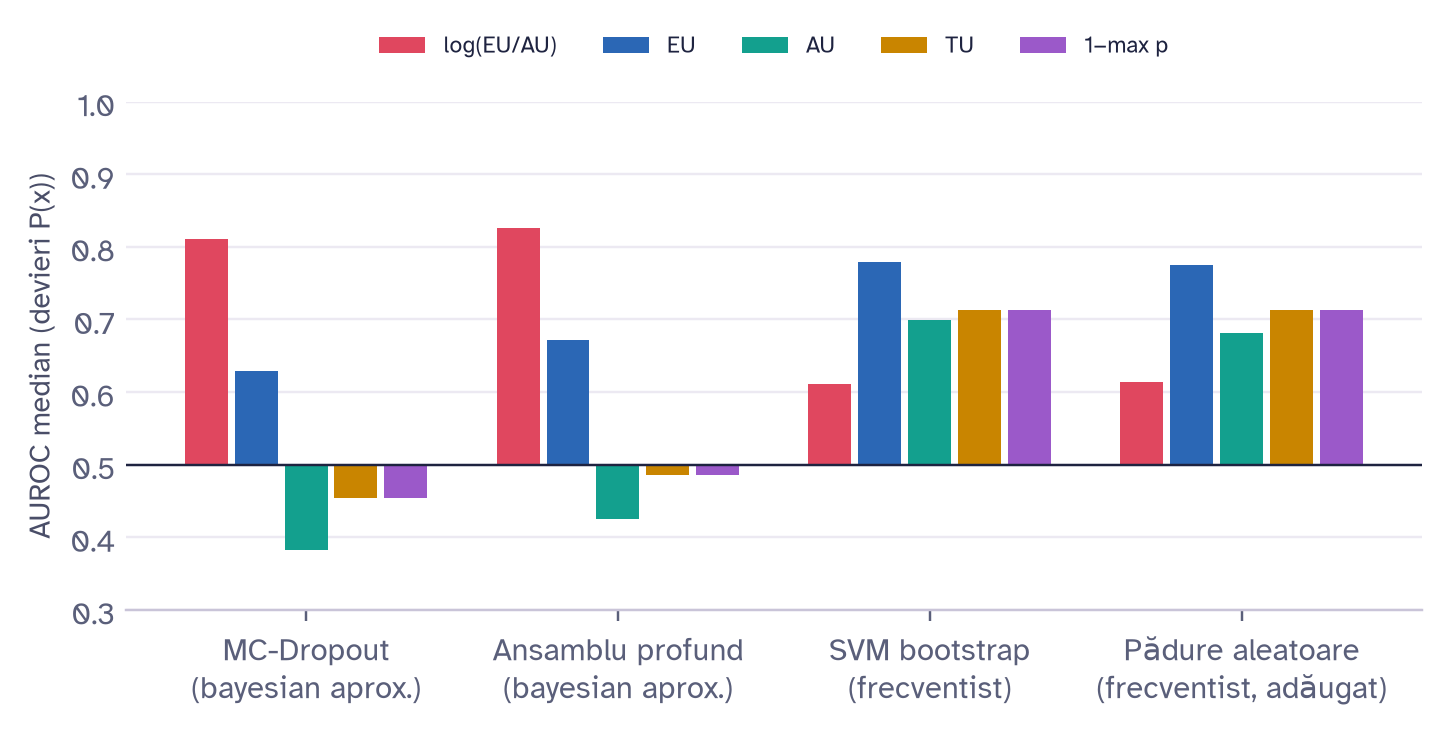
\includegraphics[width=13.5cm]{figures/fig7_bayes_vs_freq.png}
\caption{AUROC median al semnalelor pentru modelele bayesiene și frecventiste}
\end{figure}

\textbf{H1 nu este confirmată în forma sa tare.} Alarma pe LR vine mai
devreme decât DDM, ADWIN și PH pe eroare (diferențe mediane de 129, 268
și 99 de înregistrări, \(p\le0.007\)), dar precede scăderea vizibilă
doar în 51 \% din cele 53 de rulări relevante (avans median 30, interval
de încredere 95 \% {[}−25; 151{]}, \(p_{Holm}=0.24\)). Testul KS pe
intrări avertizează mai des pe aceste devieri sintetice, însă pe fluxul
Elec2 produce 148 de alarme, față de 7 pentru PH pe LR. Pe Elec2, LR
variază împreună cu eroarea (\(r=0.30\)), fără a o anticipa. Fig. 4
arată că detectoarele bazate pe eroare aproape niciodată nu avertizează
înaintea scăderii vizibile, deoarece urmăresc chiar eroarea.

\begin{figure}[H]\centering
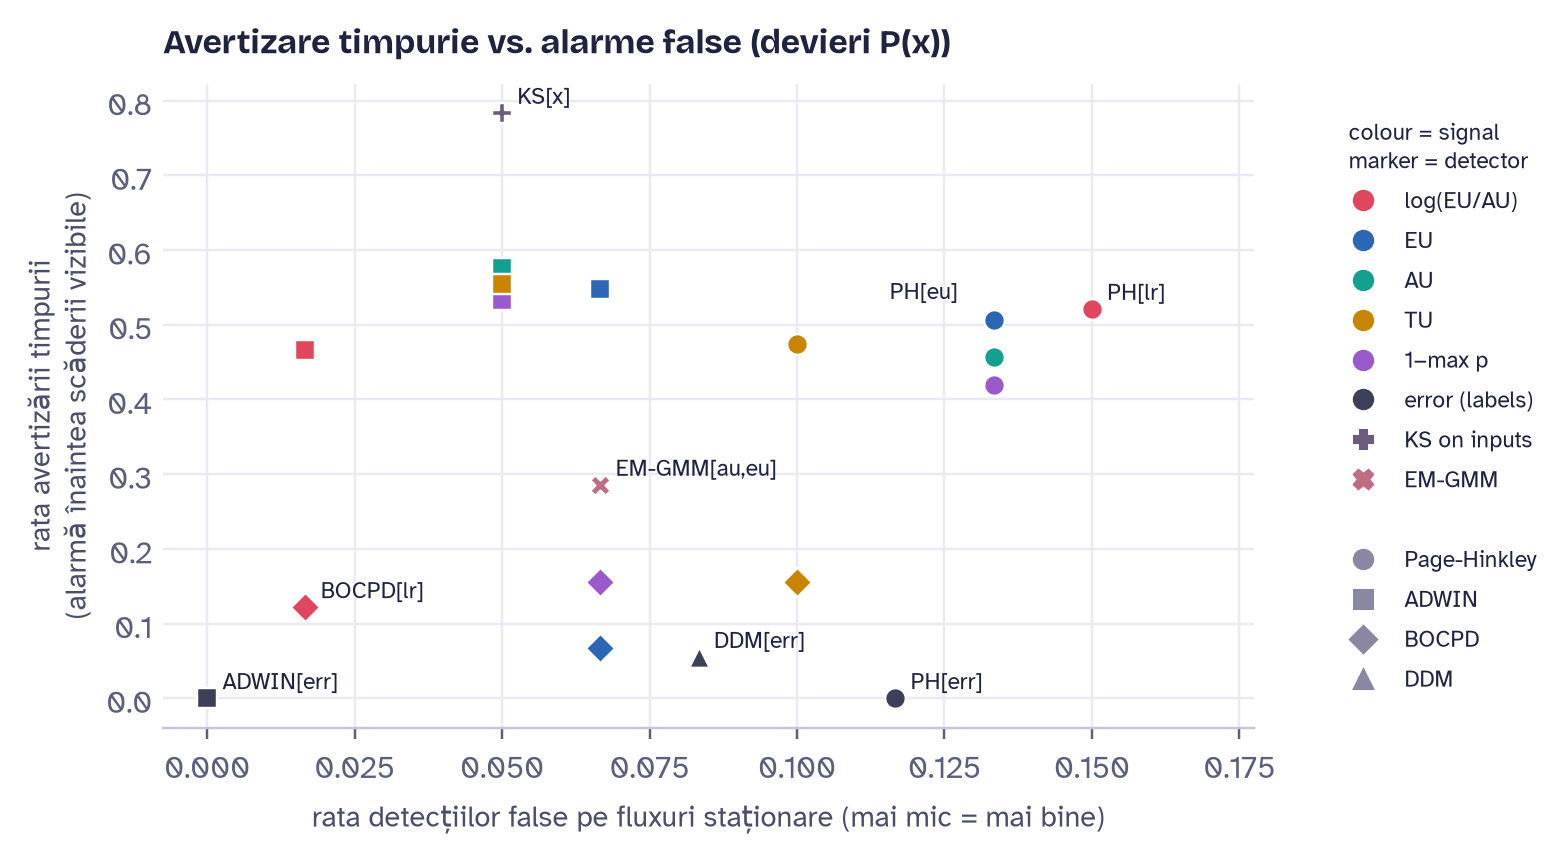
\includegraphics[width=15cm]{figures/fig3_tradeoff.png}
\caption{Rata avertizării timpurii față de rata alarmelor false pe fluxuri staționare, pentru toți detectorii}
\end{figure}

\textbf{H4 este confirmată pentru SHAP și infirmată pentru LIME} (Fig.
5). KernelSHAP și GradientSHAP plasează trăsăturile deviate în vârful
clasamentului (rang normalizat 0.78--0.92, \(p_{Holm}\le0.03\);
precizie@k până la 0.65 față de 0.08 la întâmplare), iar explicațiile
lor își pierd stabilitatea după alarmă. LIME rămâne la nivelul
hazardului.

\begin{figure}[H]\centering
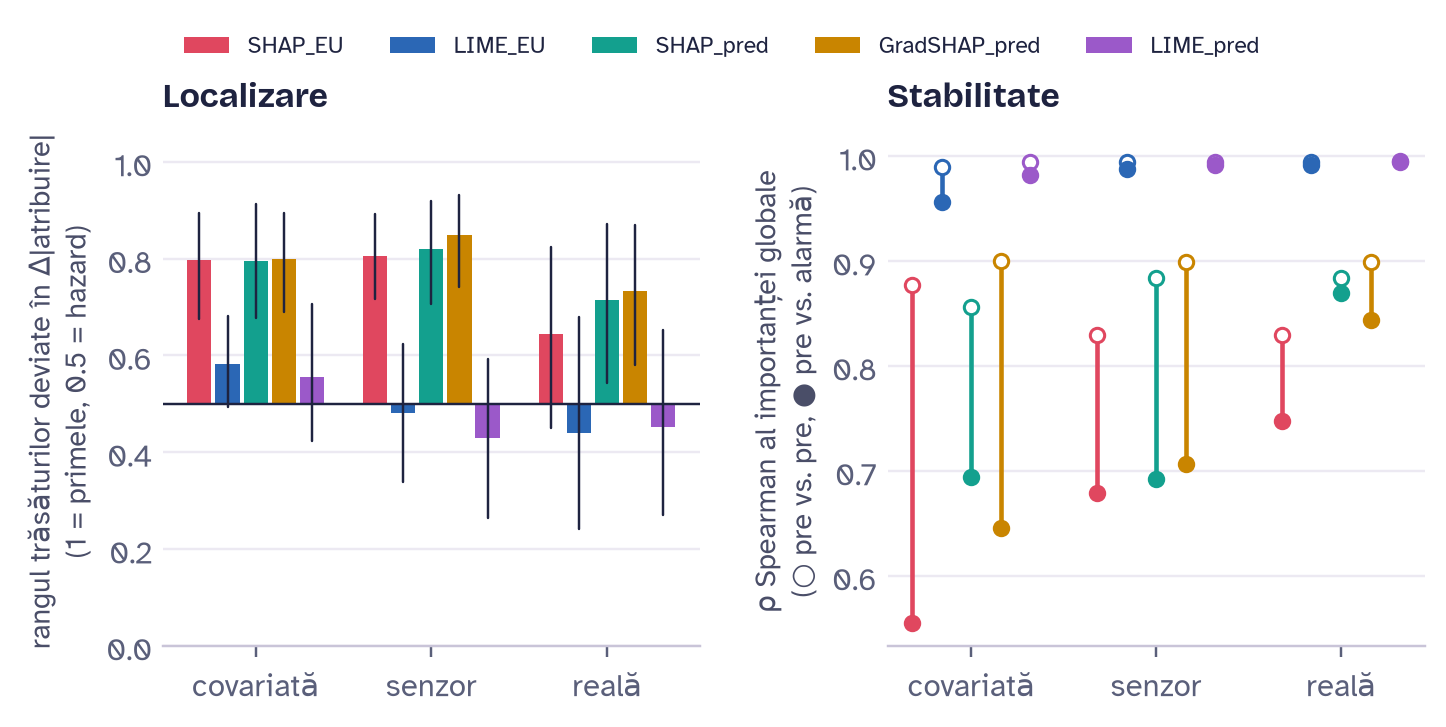
\includegraphics[width=16cm]{figures/fig5_xai.png}
\caption{Localizarea trăsăturilor deviate și stabilitatea explicațiilor SHAP și LIME}
\end{figure}

Pentru echipele care operează modele în producție, rezultatele sugerează
patru reguli: raportul LR pentru rețele ReLU; EU singur pentru modele cu
nucleu sau arbori; un eșantion etichetat periodic pentru devierea
\(P(y\mid x)\), pe care incertitudinea nu o vede; și SHAP, nu LIME,
pentru explicarea alarmelor. Limitele studiului sunt caracterul
aproximativ al MC-Dropout, criticile aduse descompunerii entropice
{[}29{]}, devierile semi-sintetice și numărul de cinci semințe per
scenariu.

\hypertarget{concluzii}{%
\section{Concluzii}\label{concluzii}}

Raportul \(\log(EU/AU)\) este cel mai bun semnal de incertitudine pentru
rețelele neuronale bayesiene aproximative, deoarece AU și EU se mișcă în
sensuri opuse. Avantajul dispare la modelele frecventiste. Alarma fără
etichete precede detectoarele bazate pe eroare, dar nu în mod sigur
scăderea vizibilă a acurateței. Devierea relației \(P(y\mid x)\) este
invizibilă pentru orice semnal fără etichete. SHAP aplicat lui EU
localizează corect trăsăturile deviate, iar LIME nu. Direcții viitoare:
rețele bayesiene complete și combinarea semnalului de incertitudine cu
un test pe intrări.

\textbf{Mulțumiri.} Autorul mulțumește coordonatorului științific pentru
îndrumare. Codul sursă, datele și aplicația interactivă sunt disponibile
la {[}adresa depozitului GitHub{]}.

\hypertarget{referinux21be}{%
\section{Referințe}\label{referinux21be}}

{\raggedright
\begin{enumerate}[label=\arabic*.,leftmargin=1cm,labelsep=0.25cm,itemsep=0pt,parsep=0pt,topsep=2pt,align=left]
\item GAMA, J.; ŽLIOBAITĖ, I.; BIFET, A.; PECHENIZKIY, M.; BOUCHACHIA, A. A survey on concept drift adaptation. \textit{ACM Computing Surveys} \textbf{2014}, \textit{46}(4), Article 44, pp. 1–37, doi: 10.1145/2523813.
\item LU, J.; LIU, A.; DONG, F.; GU, F.; GAMA, J.; ZHANG, G. Learning under concept drift: A review. \textit{IEEE Transactions on Knowledge and Data Engineering} \textbf{2019}, \textit{31}(12), pp. 2346–2363, doi: 10.1109/TKDE.2018.2876857.
\item GAMA, J.; MEDAS, P.; CASTILLO, G.; RODRIGUES, P. Learning with drift detection. In \textit{Advances in Artificial Intelligence – SBIA 2004}, Proceedings of the 17th Brazilian Symposium on Artificial Intelligence, São Luis, Brazil, 29 September – 1 October 2004; Lecture Notes in Computer Science, vol. 3171; Springer: Berlin, Germany, 2004; pp. 286–295, doi: 10.1007/978-3-540-28645-5\_29.
\item BIFET, A.; GAVALDÀ, R. Learning from time-changing data with adaptive windowing. In \textit{Proceedings of the 2007 SIAM International Conference on Data Mining}, Minneapolis, USA, 26–28 April 2007; SIAM: Philadelphia, USA, 2007; pp. 443–448, doi: 10.1137/1.9781611972771.42.
\item PAGE, E.S. Continuous inspection schemes. \textit{Biometrika} \textbf{1954}, \textit{41}(1–2), pp. 100–115, doi: 10.1093/biomet/41.1-2.100.
\item BAIER, L.; SCHLÖR, T.; SCHÖFFER, J.; KÜHL, N. Detecting concept drift with neural network model uncertainty. In \textit{Proceedings of the 56th Hawaii International Conference on System Sciences (HICSS)}, Maui, USA, 3–6 January 2023. Disponibil online: \url{https://aisel.aisnet.org/hicss-56/da/big_data_and_analytics/6} (accesat la data de 9 octombrie 2026).
\item KENDALL, A.; GAL, Y. What uncertainties do we need in Bayesian deep learning for computer vision? In \textit{Advances in Neural Information Processing Systems 30}, Proceedings of NeurIPS 2017, Long Beach, USA, 4–9 December 2017; Curran Associates: Red Hook, USA, 2017; pp. 5574–5584.
\item DEPEWEG, S.; HERNÁNDEZ-LOBATO, J.M.; DOSHI-VELEZ, F.; UDLUFT, S. Decomposition of uncertainty in Bayesian deep learning for efficient and risk-sensitive learning. In \textit{Proceedings of the 35th International Conference on Machine Learning}, Stockholm, Sweden, 10–15 July 2018; Proceedings of Machine Learning Research, vol. 80; PMLR, 2018; pp. 1184–1193.
\item HÜLLERMEIER, E.; WAEGEMAN, W. Aleatoric and epistemic uncertainty in machine learning: an introduction to concepts and methods. \textit{Machine Learning} \textbf{2021}, \textit{110}, pp. 457–506, doi: 10.1007/s10994-021-05946-3.
\item GAL, Y.; GHAHRAMANI, Z. Dropout as a Bayesian approximation: Representing model uncertainty in deep learning. In \textit{Proceedings of the 33rd International Conference on Machine Learning}, New York, USA, 19–24 June 2016; Proceedings of Machine Learning Research, vol. 48; PMLR, 2016; pp. 1050–1059.
\item LAKSHMINARAYANAN, B.; PRITZEL, A.; BLUNDELL, C. Simple and scalable predictive uncertainty estimation using deep ensembles. In \textit{Advances in Neural Information Processing Systems 30}, Proceedings of NeurIPS 2017, Long Beach, USA, 4–9 December 2017; Curran Associates: Red Hook, USA, 2017; pp. 6402–6413.
\item BREIMAN, L. Random forests. \textit{Machine Learning} \textbf{2001}, \textit{45}(1), pp. 5–32, doi: 10.1023/A:1010933404324.
\item SHAKER, M.H.; HÜLLERMEIER, E. Aleatoric and epistemic uncertainty with random forests. In \textit{Advances in Intelligent Data Analysis XVIII}, Proceedings of IDA 2020, Konstanz, Germany, 27–29 April 2020; Lecture Notes in Computer Science, vol. 12080; Springer: Cham, Switzerland, 2020; pp. 444–456, doi: 10.1007/978-3-030-44584-3\_35.
\item YEH, I.-C.; LIEN, C.-H. The comparisons of data mining techniques for the predictive accuracy of probability of default of credit card clients. \textit{Expert Systems with Applications} \textbf{2009}, \textit{36}(2), pp. 2473–2480, doi: 10.1016/j.eswa.2007.12.020.
\item IBM. Telco Customer Churn (set de date). Disponibil online: \url{https://github.com/IBM/telco-customer-churn-on-icp4d} (accesat la data de 9 octombrie 2026).
\item HARRIES, M. \textit{SPLICE-2 Comparative Evaluation: Electricity Pricing}; Technical Report; University of New South Wales: Sydney, Australia, 1999.
\item STREET, W.N.; KIM, Y. A streaming ensemble algorithm (SEA) for large-scale classification. In \textit{Proceedings of the 7th ACM SIGKDD International Conference on Knowledge Discovery and Data Mining}, San Francisco, USA, 26–29 August 2001; ACM: New York, USA, 2001; pp. 377–382, doi: 10.1145/502512.502568.
\item MONTIEL, J.; HALFORD, M.; MASTELINI, S.M.; BOLMIER, G.; SOURTY, R.; VAYSSE, R.; et al. River: machine learning for streaming data in Python. \textit{Journal of Machine Learning Research} \textbf{2021}, \textit{22}(110), pp. 1–8.
\item ADAMS, R.P.; MACKAY, D.J.C. Bayesian online changepoint detection. \textit{arXiv preprint} \textbf{2007}, arXiv:0710.3742.
\item DEMPSTER, A.P.; LAIRD, N.M.; RUBIN, D.B. Maximum likelihood from incomplete data via the EM algorithm. \textit{Journal of the Royal Statistical Society: Series B (Methodological)} \textbf{1977}, \textit{39}(1), pp. 1–38, doi: 10.1111/j.2517-6161.1977.tb01600.x.
\item RABANSER, S.; GÜNNEMANN, S.; LIPTON, Z.C. Failing loudly: An empirical study of methods for detecting dataset shift. In \textit{Advances in Neural Information Processing Systems 32}, Proceedings of NeurIPS 2019, Vancouver, Canada, 8–14 December 2019; Curran Associates: Red Hook, USA, 2019.
\item LUNDBERG, S.M.; LEE, S.-I. A unified approach to interpreting model predictions. In \textit{Advances in Neural Information Processing Systems 30}, Proceedings of NeurIPS 2017, Long Beach, USA, 4–9 December 2017; Curran Associates: Red Hook, USA, 2017; pp. 4765–4774.
\item RIBEIRO, M.T.; SINGH, S.; GUESTRIN, C. „Why should I trust you?”: Explaining the predictions of any classifier. In \textit{Proceedings of the 22nd ACM SIGKDD International Conference on Knowledge Discovery and Data Mining}, San Francisco, USA, 13–17 August 2016; ACM: New York, USA, 2016; pp. 1135–1144, doi: 10.1145/2939672.2939778.
\item HOLM, S. A simple sequentially rejective multiple test procedure. \textit{Scandinavian Journal of Statistics} \textbf{1979}, \textit{6}(2), pp. 65–70.
\item SCHUIRMANN, D.J. A comparison of the two one-sided tests procedure and the power approach for assessing the equivalence of average bioavailability. \textit{Journal of Pharmacokinetics and Biopharmaceutics} \textbf{1987}, \textit{15}(6), pp. 657–680, doi: 10.1007/BF01068419.
\item KÜNSCH, H.R. The jackknife and the bootstrap for general stationary observations. \textit{The Annals of Statistics} \textbf{1989}, \textit{17}(3), pp. 1217–1241, doi: 10.1214/aos/1176347265.
\item DERSIMONIAN, R.; LAIRD, N. Meta-analysis in clinical trials. \textit{Controlled Clinical Trials} \textbf{1986}, \textit{7}(3), pp. 177–188, doi: 10.1016/0197-2456(86)90046-2.
\item HEIN, M.; ANDRIUSHCHENKO, M.; BITTERWOLF, J. Why ReLU networks yield high-confidence predictions far away from the training data and how to mitigate the problem. In \textit{Proceedings of the IEEE/CVF Conference on Computer Vision and Pattern Recognition (CVPR)}, Long Beach, USA, 16–20 June 2019; IEEE: Piscataway, USA, 2019; pp. 41–50, doi: 10.1109/CVPR.2019.00013.
\item WIMMER, L.; SALE, Y.; HOFMAN, P.; BISCHL, B.; HÜLLERMEIER, E. Quantifying aleatoric and epistemic uncertainty in machine learning: Are conditional entropy and mutual information appropriate measures? In \textit{Proceedings of the 39th Conference on Uncertainty in Artificial Intelligence}, Pittsburgh, USA, 31 July – 4 August 2023; Proceedings of Machine Learning Research, vol. 216; PMLR, 2023; pp. 2282–2292.
\end{enumerate}\par}

\newpage\vspace*{2cm}\begin{center}\textbf{Declarație de originalitate și asumare a responsabilității}\end{center}\vspace{6pt}{\setlength{\parindent}{0pt}\setstretch{1.5}
Subsemnatul(a), în calitate de autor corespondent, declar că lucrarea cu titlul „Descompunerea bayesiană a incertitudinii pentru avertizarea timpurie a devierii conceptuale, validată prin XAI” este originală, reprezintă rezultatul activității autorilor și că toate sursele bibliografice utilizate sunt citate corespunzător. Îmi asum responsabilitatea pentru integritatea lucrării și corectitudinea informațiilor prezentate în această lucrare în numele tuturor coautorilor.\par}\vspace{1.5cm}{\setlength{\parindent}{0pt}Numele și prenumele: \rule{6cm}{0.4pt}\\[14pt]Semnătura: \rule{6cm}{0.4pt}\\[14pt]Data: \rule{6cm}{0.4pt}\par}
\end{document}
